%%%%%%%%%%%%%%%%%%%%%%%%%%%%%%%%%%%%%%%%%
% Short Sectioned Assignment LaTeX Template Version 1.0 (5/5/12)
% This template has been downloaded from: http://www.LaTeXTemplates.com
% Original author:  Frits Wenneker (http://www.howtotex.com)
% License: CC BY-NC-SA 3.0 (http://creativecommons.org/licenses/by-nc-sa/3.0/)
%%%%%%%%%%%%%%%%%%%%%%%%%%%%%%%%%%%%%%%%%

%----------------------------------------------------------------------------------------
%   PACKAGES AND OTHER DOCUMENT CONFIGURATIONS
%----------------------------------------------------------------------------------------

\documentclass[10pt,a4paper,spanish]{article}

% ---- Entrada y salida de texto -----

\usepackage[spanish]{babel} 
\usepackage[T1]{fontenc} % Use 8-bit encoding that has 256 glyphs
\usepackage[utf8]{inputenc}
\usepackage{cite}
% \usepackage{spreadtab}
% \usepackage{fourier} % Use the Adobe Utopia font for the document - comment this line to return to the LaTeX default
\usepackage[usenames, dvipsnames]{color}
\usepackage[table]{xcolor}
\usepackage{colortbl}
\usepackage[bookmarks=true,colorlinks=true,linkcolor=red,citecolor=blue]{hyperref}
% \usepackage{cite}
% \usepackage[official]{eurosym}
\usepackage{tikz}
% \usepackage{pgfplots}
% \pgfplotsset{compat=1.5}

\usepackage{subfigure}

% \usepackage{pseudocode}

% ---- Otros paquetes ----
\usepackage{enumerate}
\usepackage{amsmath,amsfonts,amsthm,amssymb} % Math packages
\usepackage{graphics,graphicx} %para incluir imágenes y notas en las imágenes
% Para hacer tablas comlejas
%\usepackage{multirow}
%\usepackage{threeparttable}

\usepackage[a4paper, margin=1.3in]{geometry}


\usepackage{sectsty} % Allows customizing section commands
\allsectionsfont{\centering \normalfont\bfseries\scshape} % Make all sections centered, the default font and small caps
\usepackage{fancyhdr}
\pagestyle{fancy}
%con esto nos aseguramos de que las cabeceras de capítulo y de sección vayan en minúsculas

\renewcommand{\sectionmark}[1]{%
      \markright{\thesection\ #1}}
\fancyhf{} %borra cabecera y pie actuales
\fancyhead[LE,RO]{{\bfseries Práctica 2}}
\fancyhead[LO]{\bfseries Marta Gómez}
\fancyfoot[C]{\thepage{}}
\renewcommand{\headrulewidth}{0.5pt}
\renewcommand{\footrulewidth}{0pt}
\addtolength{\headheight}{0.5pt} %espacio para la raya
\fancypagestyle{plain}{%
      \fancyhead{} %elimina cabeceras en páginas "plain"
      \renewcommand{\headrulewidth}{0pt} %así como la raya
}

\numberwithin{equation}{section} % Number equations within sections (i.e. 1.1, 1.2, 2.1, 2.2 instead of 1, 2, 3, 4)
\numberwithin{figure}{section} % Number figures within sections (i.e. 1.1, 1.2, 2.1, 2.2 instead of 1, 2, 3, 4)
\numberwithin{table}{section} % Number tables within sections (i.e. 1.1, 1.2, 2.1, 2.2 instead of 1, 2, 3, 4)

\setlength\parindent{0pt} % Removes all indentation from paragraphs - comment this line for an assignment with lots of text
\setlength{\parskip}{1ex plus 0.5ex minus 0.2ex}


\theoremstyle{plain}
\newtheorem{exe}{Ejercicio}[section] % reset theorem numbering for each section

\theoremstyle{definition}
\newtheorem{sol}{Solución}[section]

\newcommand{\horrule}[1]{\rule{\linewidth}{#1}} % Create horizontal rule command with 1 argument of height

%----------------------------------------------------------------------------------------
%   TÍTULO Y DATOS DEL ALUMNO
%----------------------------------------------------------------------------------------

\title{
\normalfont \normalsize 
{\bf Redes y Sistemas Complejos} \\ Curso 2016-2017 \\ [25pt] % Your university, school and/or department name(s)
\horrule{0.5pt} \\[0.4cm] % Thin top horizontal rule
\huge \textsc{Práctica 2: \\ Procedimientos generales de \\ las redes mediante \textit{Gephi} y \\ simuladores en \textit{Netlogo}} \\ % The assignment title
\horrule{2pt} \\[0.5cm] % Thick bottom horizontal rule
}

\author{\textit{Marta Gómez Macías}} %\\ \texttt{mgmacias95@correo.ugr.es} \\ 75929776Z \\[0.5cm]

% \date{\normalsize\today} % Incluye la fecha actual

% \usepackage{pdflscape}

%----------------------------------------------------------------------------------------
% DOCUMENTO
%----------------------------------------------------------------------------------------

\begin{document}
%Cambiar Cuadros por Tablas y lista de...
\renewcommand{\listtablename}{Índice de tablas}
\renewcommand{\tablename}{Tabla}

\begin{titlepage}
\begin{center}

\includegraphics[width=0.2\textwidth]{../../ugr}

\normalfont \normalsize 
{\bf Redes y Sistemas Complejos} \\ Curso 2016-2017 \\ [25pt] % Your university, school and/or department name(s)
\horrule{0.5pt} \\[0.4cm] % Thin top horizontal rule
{\huge \textsc{Práctica 2: \\ Procedimientos generales de \\ las redes mediante \textit{Gephi} y \\ simuladores en \textit{Netlogo}}} % The assignment title
\horrule{2pt} \\[0.5cm] % Thick bottom horizontal rule

{\Large \textit{Marta Gómez Macías} \\ \texttt{mgmacias95@correo.ugr.es} \\ 75929776Z \\[0.5cm]

\date{\today}} % Incluye la fecha actual
\end{center}
\end{titlepage}

\tableofcontents % para generar el índice de contenidos
\newpage

\setcounter{section}{1}
\section{Grafos}
\subsection{Componente gigante de una Red Aleatoria}
En el modelo de \textit{Netlogo} proporcionado tenemos una red aleatoria de $x$ enlaces y, en cada iteración, se genera un enlace entre dos nodos con una probabilidad uniforme, es decir, todos los nodos tienen la misma probabilidad de tener un enlace entre sí. En la \hyperref[cg80]{Figura \ref*{cg80}} muestro una evolución de la red aleatoria. Inicialmente, tenemos una red dispersa (\hyperref[cg80-1]{Figura \thesection .\ref*{cg80-1}}) donde la componente gigante está formada por menos de diez nodos. Desde el momento en el que se llega a $<k>=1$, en la \hyperref[cg80-2]{Figura \thesection .\ref*{cg80-2}}, \textbf{el tamaño de la componente gigante se incrementa mucho más rápido}. En la \hyperref[cg80-3]{Figura \thesection .\ref*{cg80-3}} vemos una representación de la red 34 iteraciones después, en esas 34 iteraciones el tamaño de la componente gigante se ha duplicado. Por último, en la \hyperref[cg80-4]{Figura \thesection .\ref*{cg80-4}} vemos el instante en el que la componente gigante ha cubierto todos los nodos de la red. Si nos fijamos en la gráfica de esta última figura, vemos que la pendiente de la misma se ha incrementado a partir del momento $<k>=1$, este incremento ha sido mucho mayor al principio (\hyperref[cg80-3]{Figura \thesection .\ref*{cg80-3}}) ya que al final de la ejecución del modelo muchos de los nuevos enlaces que surgían en cada iteración eran conexiones entre nodos de la componente gigante.

\begin{figure}[!h]
    \centering
    \mbox{
        \subfigure[Inicio de la ejecución del modelo]{
            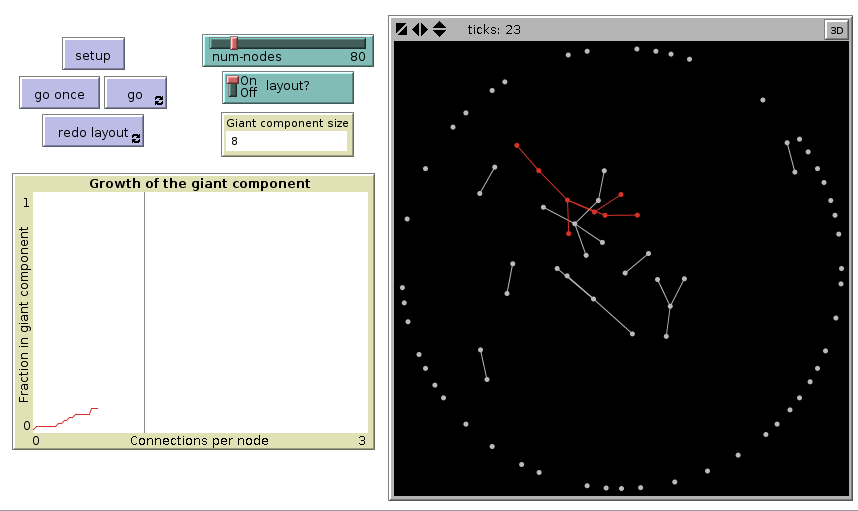
\includegraphics[width=0.5\textwidth]{cg80-1}
            \label{cg80-1}
        }
        \subfigure[Momento en el que el grado medio de los nodos del modelo llega a 1]{
            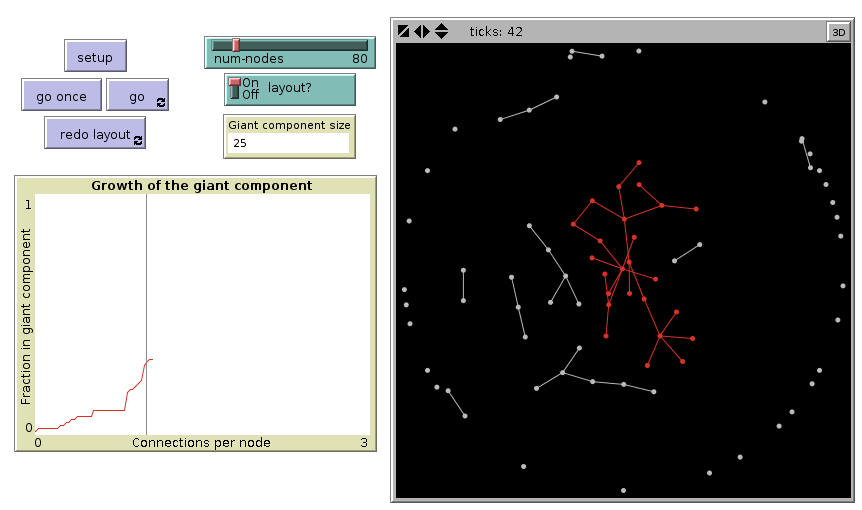
\includegraphics[width=0.5\textwidth]{cg80-2}
            \label{cg80-2}
        }
    }
    \mbox{
        \subfigure[Una vez superado el grado medio 1, el tamaño de la componente gigante se ha disparado]{
            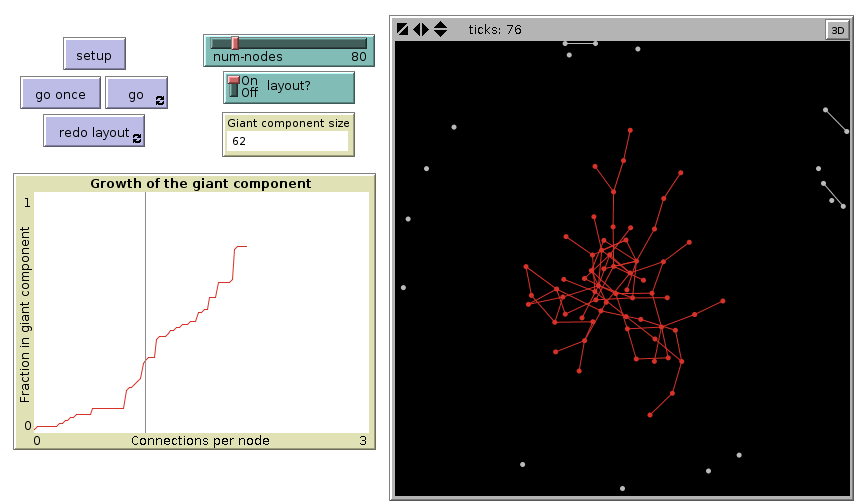
\includegraphics[width=0.5\textwidth]{cg80-3}
            \label{cg80-3}
        }
        \subfigure[Al final de la ejecución, la componente gigante ha abarcado todos los nodos de la red]{
            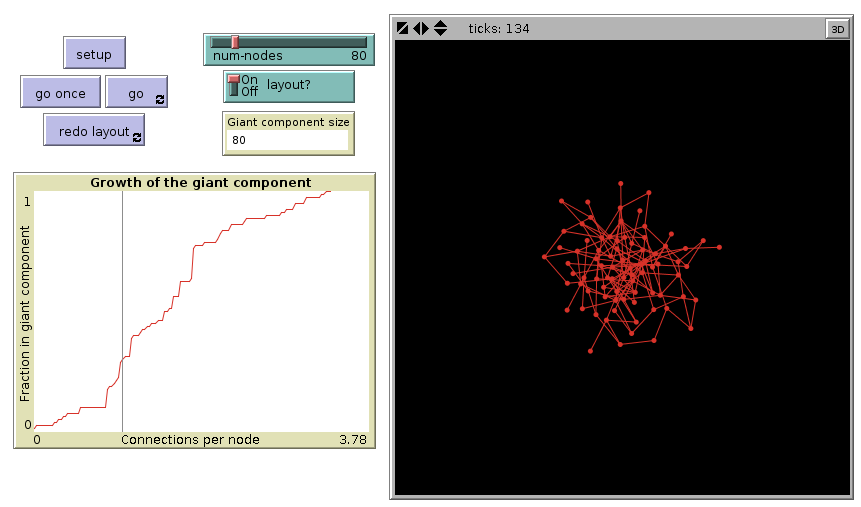
\includegraphics[width=0.5\textwidth]{cg80-4}
            \label{cg80-4}
        }
    }
    \caption{Evolución de una red aleatoria con 80 nodos}
    \label{cg80}
\end{figure}

¿A qué se debe este fenómeno? La \hyperref[cg]{ecuación \ref*{cg}} representa la proporción de nodos en la componente gigante. 

\begin{equation}
    S = 1 - e^{-<k>S}
    \label{cg}
\end{equation}

Si fijamos $S = 0$, obtenemos una transición de fase en $<k>=1$ (\hyperref[cgd]{Ecuación \ref*{cgd}}).

\begin{equation}
    \frac{d}{dS} (1 - e^{-<k>S}) = 1 \qquad\ <k> e^{-<k>S} = 1
    \label{cgd}
\end{equation}

\subsubsection{Prueba de conceptos}
\exe{Deja correr el modelo hasta el final. ¿Responde la componente gigante obtenida a las características de dicho nombre?}

\sol{Sí, de hecho, si dejamos correr el algoritmo hasta el final, $<k> = N$, por lo que tendríamos un grafo totalmente conectado donde $L = L_{max}$.}

\exe{Ejecuta el modelo de nuevo, esta vez paso a paso. Observa cómo crecen las componentes. ¿Qué ocurre cuando la curva del gráfico tiene una pendiente más pronunciada?}

\sol{La pendiente de la curva del gráfico es más pronunciada cuando \textbf{se añaden nuevos nodos a la componente gigante.} Esto es lo que se ve en la \hyperref[cg80-3]{Figura \thesection .\ref*{cg80-3}}.}

\exe{Ejecuta el modelo con un número pequeño de nodos (como 10) y observa el gráfico. ¿En qué difiere del obtenido cuando se hace funcionar el modelo con un gran número de nodos (por ejemplo, 300)? Si lo ejecutas varias veces con el mismo número de nodos, ¿cuánto varía el gráfico de una ejecución a otra?}

\sol{En la \hyperref[cgcmp]{Figura \ref*{cgcmp}} vemos una comparación de la ejecución del modelo con una red pequeña ($N = 12$) y una grande ($N = 300$). La hráfica del modelo con una red pequeña tiene muchos escalones y, además, una pendiente menor. En cambio, la gráfica del modelo con una red grande tiene una pendiente mucho mayor y es menos escalonada, debido a que el número de nodos es mayor. 

En cuanto al parecido de los gráficos en diferentes ejecuciones, tanto en redes grandes como pequeñas obtenemos gráficos muy parecidos en todas las ejecuciones. Esto se debe a que, aunque los enlaces se creen de forma aleatoria, siguen el modelo de evolución de una red aleatoria comentado anteriormente. 

\begin{figure}[!h]
\centering
\mbox{
    \subfigure[Ejecución del modelo con una red pequeña ($N = 12$)]{
        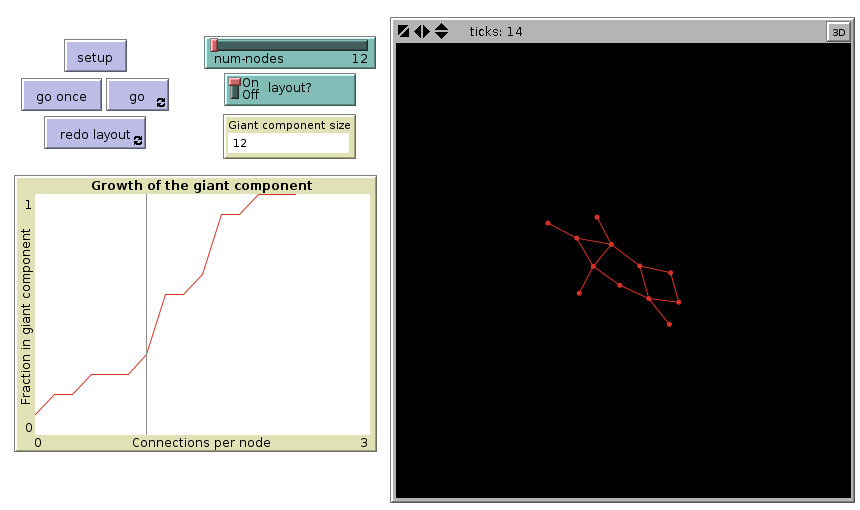
\includegraphics[width=0.5\textwidth]{cg12}
        \label{cg12}
    }
    \subfigure[Ejecución del modelo con una red grande ($N = 300$)]{
        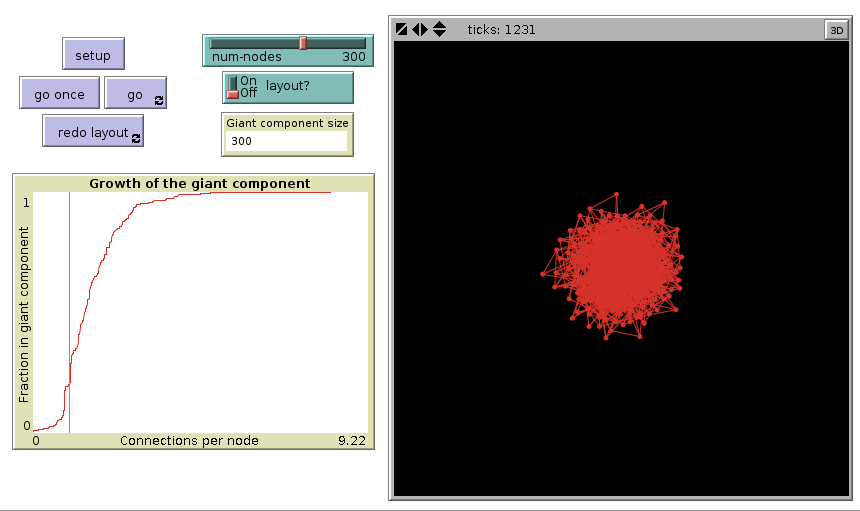
\includegraphics[width=0.5\textwidth]{cg300}
        \label{cg300}
    }
}
\caption{Comparación de la ejecución con una red pequeña y una grande}
\label{cgcmp}
\end{figure}
}

\subsubsection{Extensión del modelo}

\exe{En este momento, la probabilidad de que dos nodos cualesquiera queden conectados entre sí es la misma. ¿Puedes pensar en formas de hacer que algunos nodos sean más atractivos para conectarse que otros? ¿Cómo influiría eso en la formación de la componente gigante?}

\sol{Para hacer que unos nodos sean más atractivos que otros, haría que la probabilidad de que un nodo $n$ se conectase a otro cualquiera $n'$ dependiese del número de enlaces que tuviese $n'$. Así, los nodos con más enlaces serían más atractivos que aquellos que se encuentran aislados. Este modelo se correspondería con el \textit{Preferential Attachment}.

Esto haría que la red dejase de ser aleatoria y pasase a ser una red real con hubs (nodos a los que es más probable estar conectado) y nodos aislados, como se ve en la \hyperref[pref]{Figura \ref*{pref}}.

\begin{figure}[!h]
    \centering
    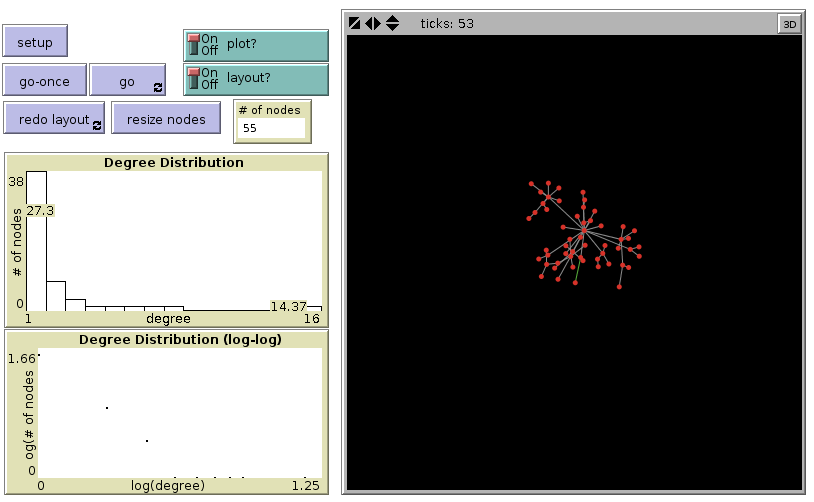
\includegraphics[width=0.5\textwidth]{pref}
    \caption{Ejecución del modelo \textit{Preferential Attachment}}
    \label{pref}
\end{figure}}

\subsection{Dos componentes gigantes de una Red Aleatoria}

En la \hyperref[2cg20]{Figura \ref*{2cg20}} vemos la evolución de la ejecución del modelo en una red con $N=40$ nodos. Añadiendo algo más de $N$ enlaces (\hyperref[2cg40-2]{Figura \thesection .\ref*{2cg40-2}}) entre las dos componentes gigantes podemos mezclarlas, tal y como se ha hecho en la \hyperref[2cg40-3]{Figura \thesection .\ref*{2cg40-3}}. 

\begin{figure}[!h]
    \centering
    \mbox{
        \subfigure[Configuración inicial de 40 nodos, 20 de cada clase]{
            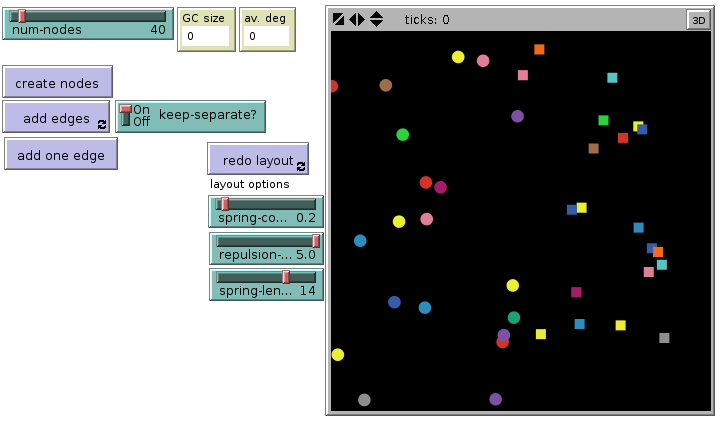
\includegraphics[width=0.5\textwidth]{2cg40}
            \label{2cg40}
        }
        \subfigure[Creación de las dos componentes gigantes separadas]{
            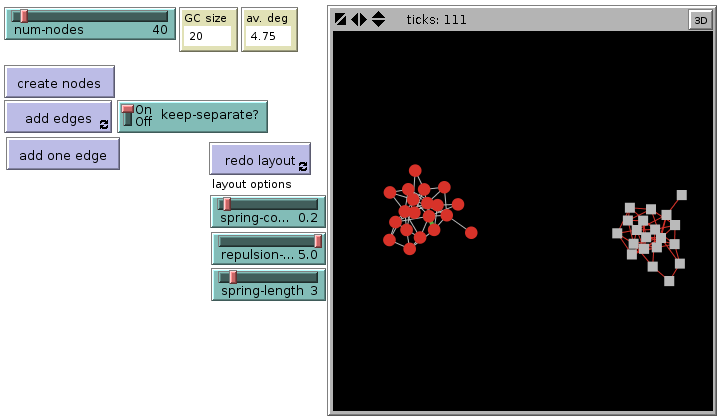
\includegraphics[width=0.5\textwidth]{2cg40-1}
            \label{2cg40-1}
        }
    }
    \mbox{
        \subfigure[Tras 60 clicks a \textit{add one edge}, tenemos bastantes enlaces conectando las dos componentes]{
            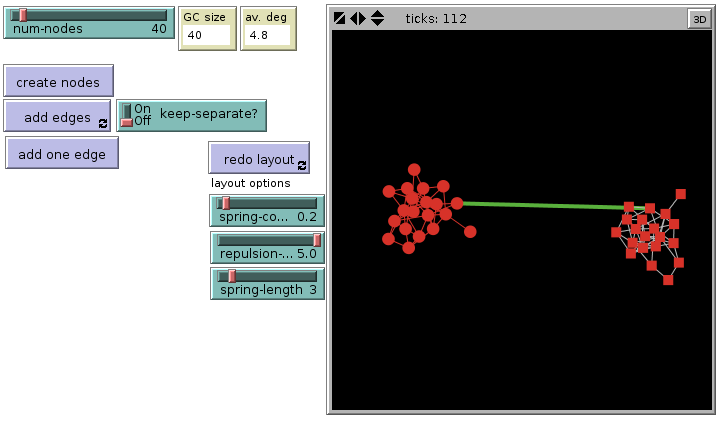
\includegraphics[width=0.5\textwidth]{2cg40-2}
            \label{2cg40-2}
        }
        \subfigure[Si revisualizamos la red, ambas componentes gigantes quedan mezcladas]{
            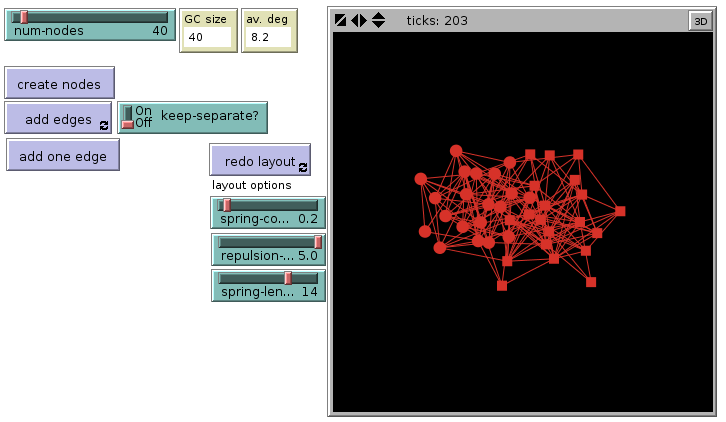
\includegraphics[width=0.5\textwidth]{2cg40-3}
            \label{2cg40-3}
        }
    }
    \caption{Mezclando dos componentes gigantes de 20 nodos cada una}
    \label{2cg20}
\end{figure}

\subsubsection{Aspectos importantes}

\exe{¿Tiene sentido que los grafos aleatorios sólo generen una componente gigante?}

\sol{Sí, ya que la evolución de de una red aleatoria tiende a formar una única componente gigante:

\begin{enumerate}[$\qquad\ \bullet$]
    \item En el \textbf{régimen subcrítico}, no existe ninguna componente gigante, sino que hay clústers aislados.
    \item En el \textbf{régimen crítico}, aparece una única componente gigante, que contiene una fracción pequeña de nodos.
    \item En el \textbf{régimen supercrítico} hay una única componente gigante real. Este régimen se mantiene hasta que todos los nodos son absorbidos por esta componente gigante.
    \item En el \textbf{régimen conectado}, para valores grandes de $p$ la componente gigante absorbe todos los nodos y componentes. En este estado la red sigue siendo dispersa.
\end{enumerate}}

\end{document}
